\chapter{Event Selection}

The main event selection for this analysis is based on a standard cut-flow selection used within ATLAS to select high energy di-electron events. Following will be the basic outline of each requirement an event must satisfy followed by a small discussion of optimisations done to some cuts for this analysis. Finally a discussion of corrections is included spanning minor variable corrections to data obtained by performance groups after reconstruction and more substantial corrections to MC samples to correctly estimate run conditions.
The following analysis selection is applied equally the data and MC background samples unless were noted.


\section{Analysis Selection}

The following selection is made to all data and MC events for this analysis. Before selection several data flags are checked to insure full operation of the detector at time of data taking. 

{\bf Event Selection}
\begin{itemize}
\item Event is required have passed the chosen unprescaled electron trigger (EF\_g35\_loose\_g25\_loose).
\item Each event is required to contain at least one reconstructed primary vertex with at least 2 traceable charged tracks.
\end{itemize}


{\bf Electron Selection}
\begin{itemize}
\item Electron $|\eta| < 2.47$ and not lie within the detector crack region $1.37 \leq |\eta| \leq 1.52$ due to a decreased energy resolution.
\item Each electron is required to have a transverse momentum ($p_{T}$) greater than 30 GeV with the highest $p_{T}$ electron lying above 40 GeV.
\item Electrons are required to pass identification criteria on the transverse shower shape, the longitudinal leakage into the hadronic calorimeter, and the association to an inner detector track, defined together as a medium++ electron identification (see section \ref{sec:ReconElec}).
\end{itemize}


{\bf Dielectron Selection}
\begin{itemize}
\item Selection of two highest $p_{T}$ electrons left in event.
\item Lead Isolation (A cone around the candidate in the calorimeter is required to have  $< 0.007~\times~E_{T}$\\$+~5.0~GeV$ deposited in it) of the highest $p_{T}$ electron in the event is used to suppress jet's background. 
\item Sub-leading Isolation (A cone around the candidate in the calorimeter is required to have  $< 0.0022$\\$~\times~E_{T}~+~6.0~GeV$ deposited in it) of the highest $p_{T}$ electron in the event is used to suppress more jet's background. 
\item Dielectron invariant mass (m$_{ee}$) is required to be greater than or equal 80 GeV.
\item Opposite sign requirement. Require both electrons to have opposite charge.
\end{itemize}




\section{Isolation Requirement}

It was decided a re-investigation of the isolation requirement was needed, updating the cut from its previous iteration in the di-electron analysis on 2011 ATLAS data. The previous threshold was a flat, less than 7 GeV, cut on the $p_{T}$ corrected (define pT corrected) electro-magnetic calorimeter cluster isolation (definition probably required) of the highest $p_{T}$ electron in the selected pair. The first investigation was to see how this cut performed in the selection of MC signal at 8 TeV centre of mass energy. Due to the better statistics found in the $DY{\rightarrow}ee$ MC sample and this being an irreducible background and therefore indistinguishable from the signal this was used in the following investigation.

It can be seen in fig. \# that this flat cut of 7 GeV causes an increasing efficiency loss at high energy and was deemed unsuitably high for this iteration of the analysis due to the higher reach in energy expected from the higher centre of mass energy. Two methods that could be used in conjunction were proposed to solve this issue as well as the possibility of introducing a requirement on the second highest energy electron in our selected pair.

The first alternative was a different algorithm of calculating the isolation variable, topo isolation (definition required). This was deemed unsuitable after a short investigation due the similarity of distribution of final result and problems with the implementation of this algorithm in ATLAS reconstruction code. (remember and find out the exact reason)

The second possibility was an isolation requirement varying with energy. Fig. \ref{fig:C5_leadIso_vs_leadpT} shows the distribution of DY MC events in $E_{T}$ and cluster isolation. It can be seen that electrons become less isolated under this definition of isolation as energy of the electron increases. This is to be expected as higher energy electrons produce larger showers in the EM calorimeter and so are less well restrained to only a few colorimeter cells in the electron shower. 

   \begin{figure}[h]
      \begin{center}
      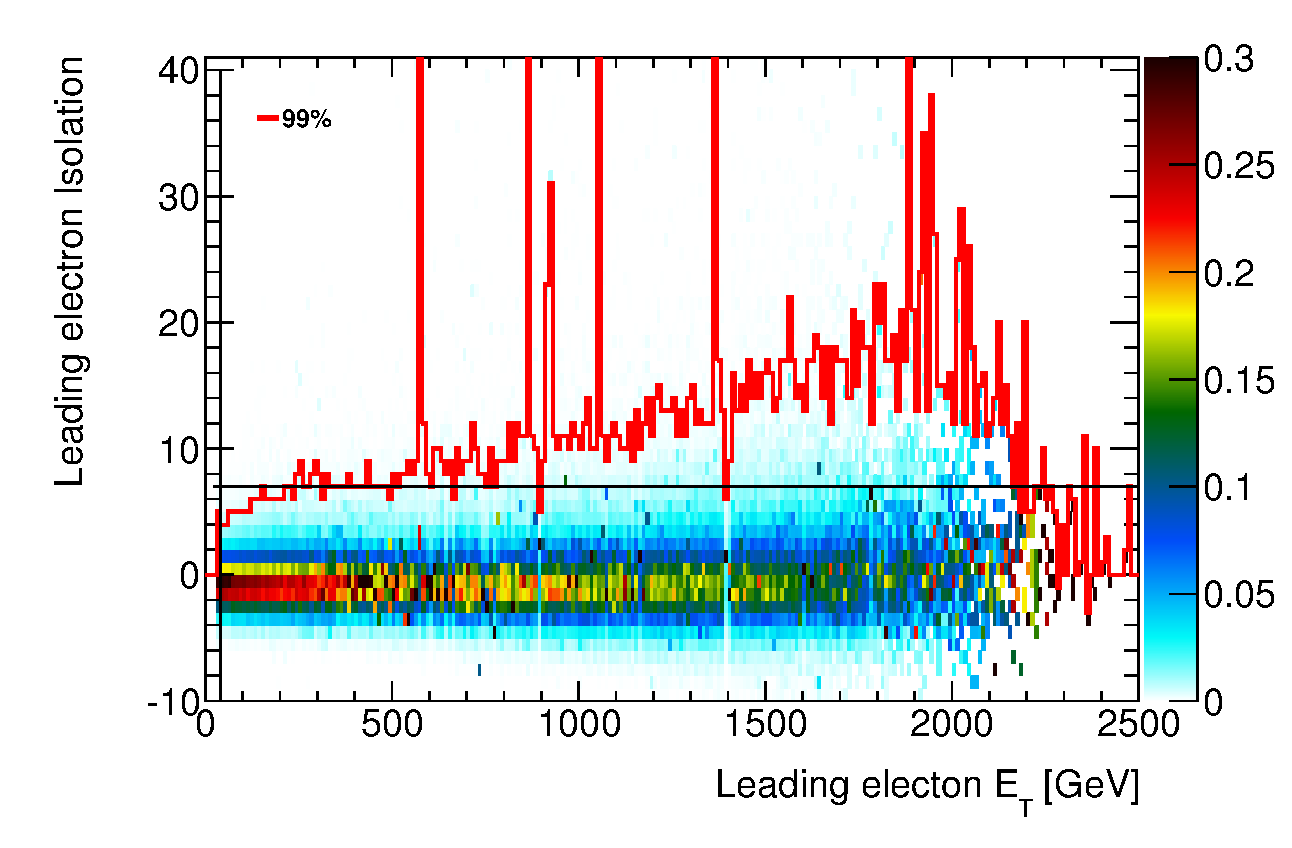
\includegraphics[scale=0.7]{images/C5_leadIso_vs_leadpT.eps}
      \end{center}
   \caption{Distribution of DY MC in $E_{T}$ and cluster isolation for the highest energy electon. Colour density shows the fraction of electons from that $E_{T}$ coulum found in cell. The red line shows the 99\% acceptance point of electrons in the $E_{T}$ coloum. While the Black vertical and horizontal lines show the $p_{T}$ and old isolation cut respectivly.}
   \label{fig:C5_leadIso_vs_leadpT}
   \end{figure}


In order to define a requirement varying in pT the 99\% acceptance point for each pT column was looked at and a 1st order polynomial fit to these points by eye was done. The 99\% acceptance points can be seen in fig. \ref{fig:C5_leadIso_vs_leadpT_proposal} as well as the estimated fit which would form the cut. The same thing was looked at for the second highest pT electron and can be seen in fig. \ref{fig:C5_subIso_vs_subpT_proposal}.


   \begin{figure}[h]
      \begin{center}
      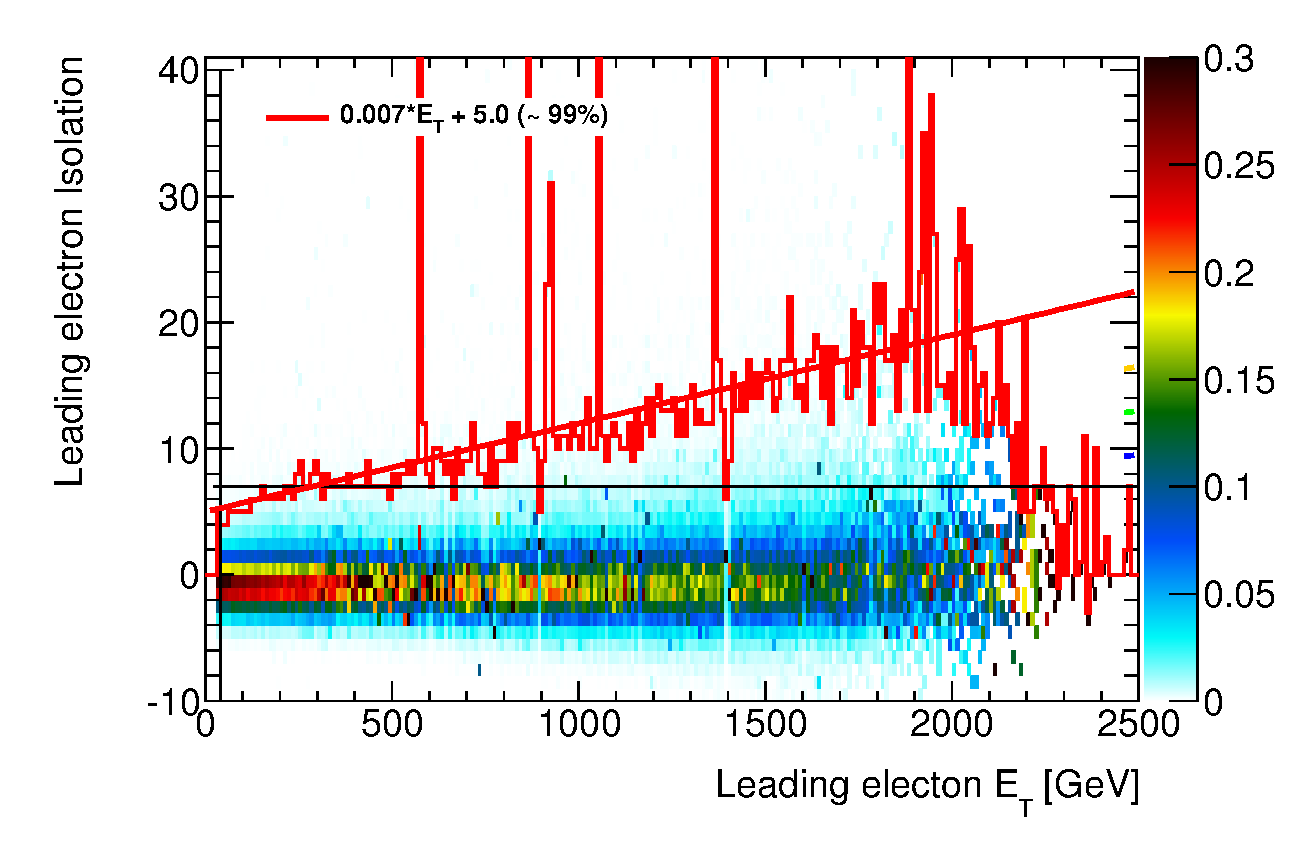
\includegraphics[scale=0.7]{images/C5_leadIso_vs_leadpT_proposal.eps}
      \end{center}
   \caption{Similar plot to Fig. \ref{fig:C5_leadIso_vs_leadpT} but with a fit 99\% as a possible issolation requirment.}
   \label{fig:C5_leadIso_vs_leadpT_proposal}
   \end{figure}


   \begin{figure}[h]
      \begin{center}
      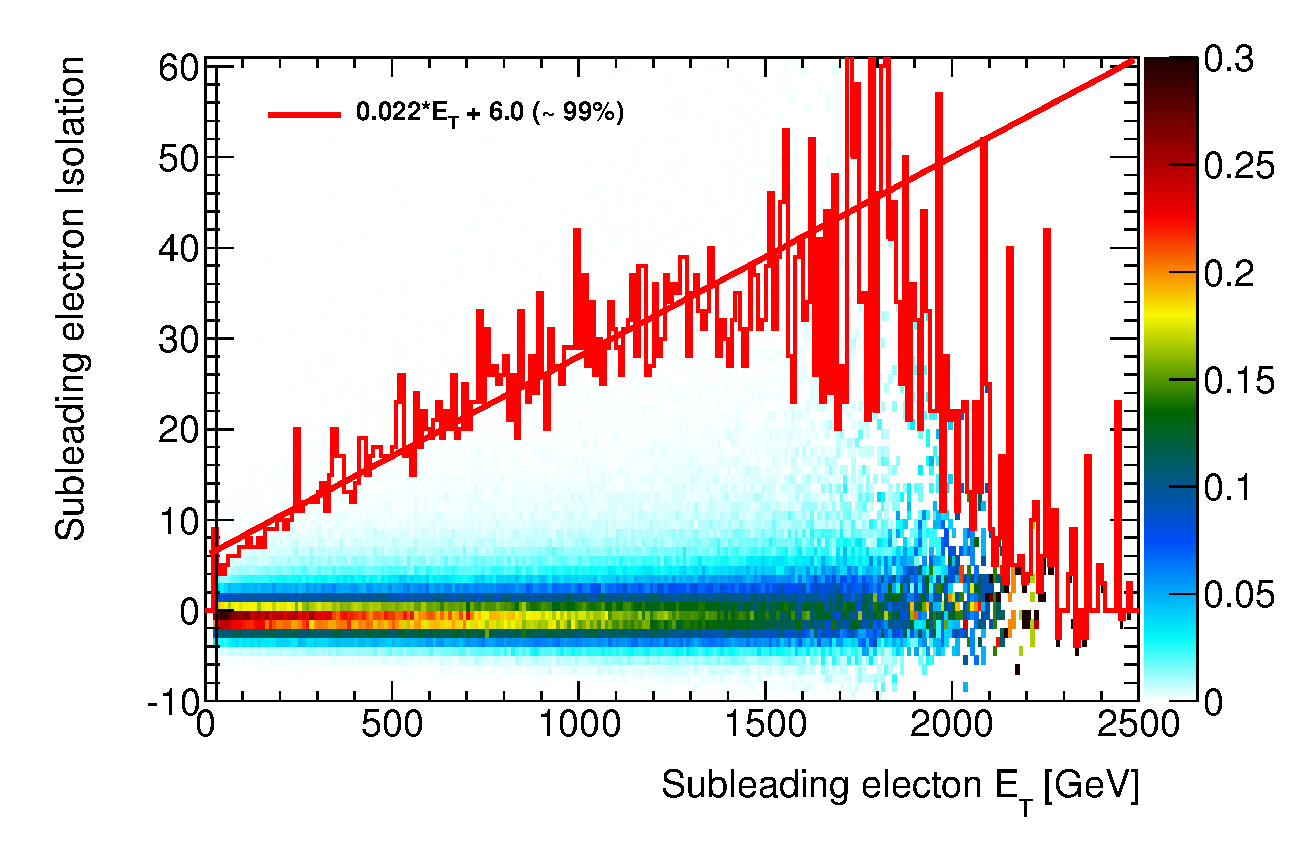
\includegraphics[scale=0.7]{images/C5_subIso_vs_subpT_proposal.eps}
      \end{center}
   \caption{Similar plot to Fig. \ref{fig:C5_leadIso_vs_leadpT_proposal} but for second highest energy electrons after the requirment proposed in Fig. \ref{fig:C5_leadIso_vs_leadpT_proposal} is applied.}
   \label{fig:C5_subIso_vs_subpT_proposal}
   \end{figure}



The two first order polynomials shown here correspond to isolation requirements of;
   \begin{center}
   $Lead~Isolation < 0.007\times~E_{T}~+~5.0~GeV$\\
   $Subleading~Isolation < 0.022\times~E_{T}~+~6.0~GeV$\\
   \end{center}
for the highest and second highest energy electrons respectively. 

An analysis of the efficiency of these cuts on signal can be seen in fig. \ref{fig:C5_lead_iso_efficiency} and fig. \ref{fig:C5_sub_iso_efficiency} where it can be seen they maintain a flat behaviour as $E_{T}$ increases.


   \begin{figure}[h]
      \begin{center}
      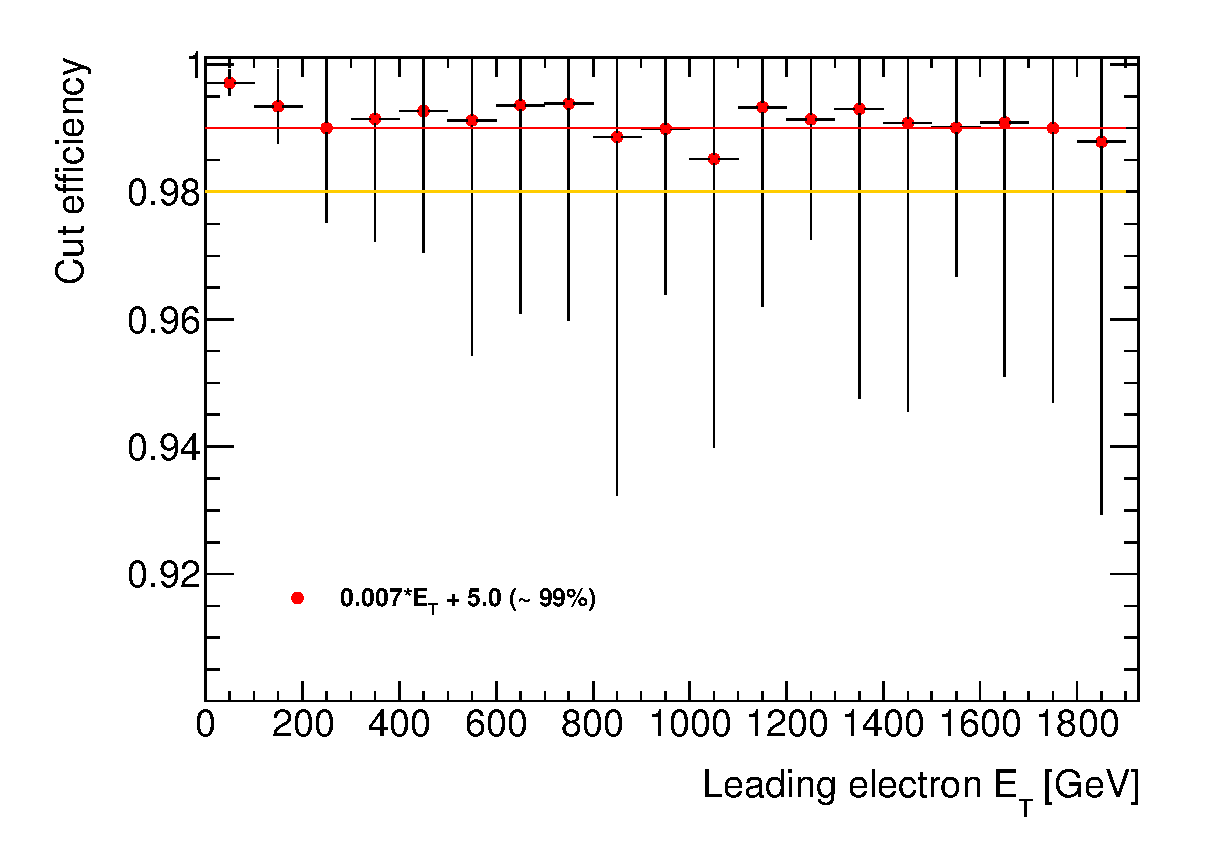
\includegraphics[scale=0.6]{images/C5_lead_iso_efficiency.eps}
      \end{center}
   \caption{Efficency of new leading electon isolation cut on selection of signal MC. Red and orange lines indicate the 99\% and 98\% efficency levels respectivly.}
   \label{fig:C5_lead_iso_efficiency}
   \end{figure}

   \begin{figure}[h]
      \begin{center}
      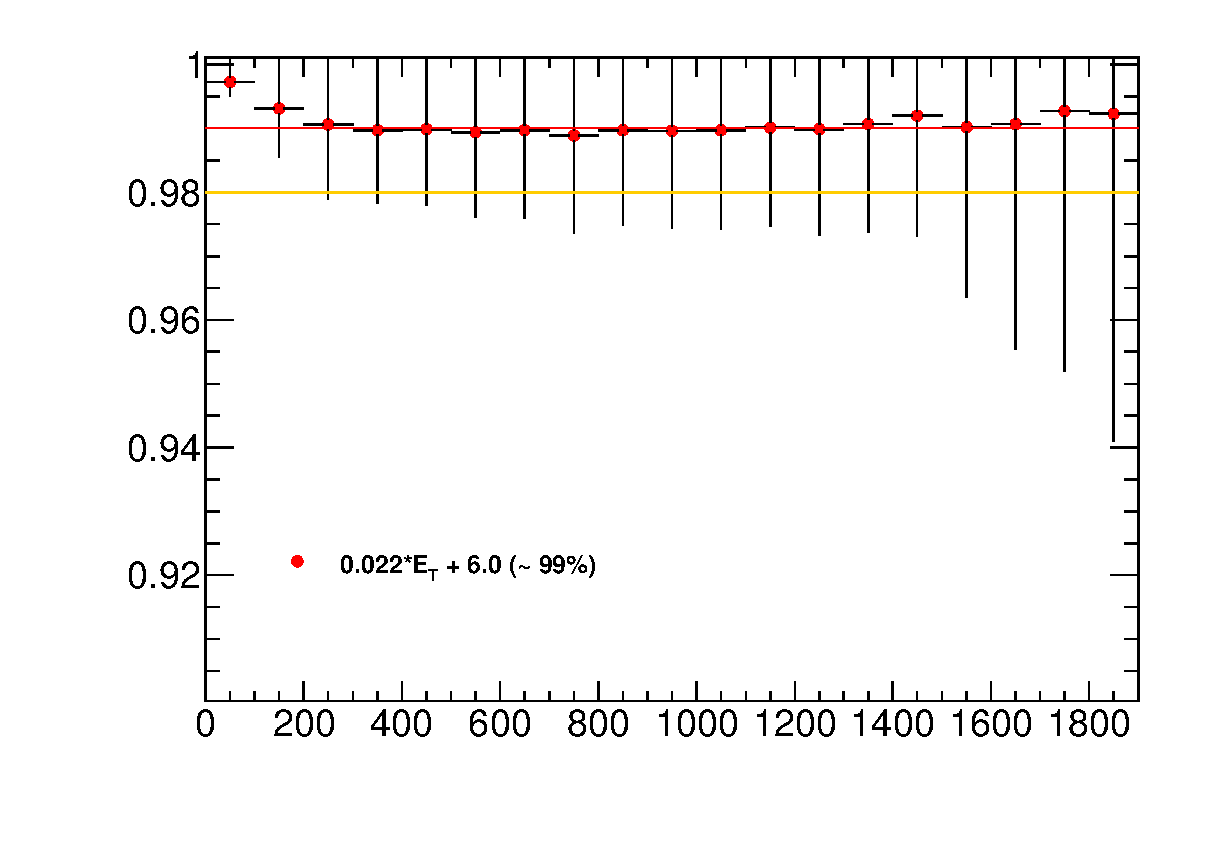
\includegraphics[scale=0.6]{images/C5_sub_iso_efficiency.eps}
      \end{center}
   \caption{Efficency of new subleading electon isolation cut oxn selection of signal MC. Red and orange lines indicate the 99\% and 98\% efficency levels respectivly.}
   \label{fig:C5_sub_iso_efficiency}
   \end{figure}

The main source of background the isolation cut is imposed to reduce is jets that fake an electron signal in the detector. It is therefore important to measure the effect of this new requirement. Jets background is estimated via a reverse ID method on data (see Section \#) and so lacks statistics at high energy. For this reason it is impossible to optimise the isolation requirement against rejection of high energy fakes as seen in fig. \#. Fig. \# shows the efficiency of acceptance of jet fakes against pT and shows a sizeable increase in efficacy over the flat cut (fig. \#) used previously. 



\section{Opposite Sign requirement}
   %\ref{Appendix}

   The opposite sign requirement was introduced to the analysis specifically due to the use of $\cos{\theta^{*}}$ in the search. As specified in section \ref{sec:CItheory} selection of the electron and not the positron is important for the definition of $\cos{\theta^{*}}$ and if reversed would dilute the asymmetry seen in the SM and CI LR signal \ref{fig:theoryAFB}. The effect of swapping charge at reconstruction level comes about due to two main effects, very high energy electrons with very straight tracks getting miss identified and hard bremsstrahlung from an electron undergoing decay to an electron pair which the wrong electron getting identified. These are not a small effect at high dielectron mass ($~ 15\%$) and so the requirement is introduced to solve the issue of miss identification. The effect of both electrons being miss identified was studied and found to have only a small chance. This requirement also does a good job in the exclusion of the Multijet background reducing by 50\% throughout the signal region. The effect of the loss of acceptance attributed to this requirement is discussed in appendix \ref{sec:oppSign}. As this requirement has some errors associated with it a systematic is introduced to accommodate it (see section \ref{sec:sys}). 


\section{Energy Scale Correction}

   During the selection process an additional correction to the energy of electrons is applied that is no included in the reconstruction. This addition results for a study done by the ATLAS electron and photon performance group at the end of the data run calibrating energies within the Z boson peak. This results in a array of energy scale corrections distributed in E$_{T}$ and $\eta$ and applied before electron selection.




\section{Selection Acceptance $\times$ Efficiency}

   Figure \ref{fig:AxE} shows the acceptance $\times$ efficiency of of the event selection at selecting DY MC events while table \ref{tab:eventEff} shows the efficiency of each part of the event selection. 



   \begin{figure}[h]
      \begin{center}
      %\includegraphics[scale=0.6]{images/}
      \end{center}
   \caption{Plot showing Acceptance $\times$ Efficiency as a function of invariant mass for DY MC events.}
   \label{fig:AxE}
   \end{figure}


   \begin {table}[h]
      \begin{center}
      \begin{tabular}{|l|c|c|}
         \hline
         \hline
         Criterion & Relative Eff [\%] & Cumulative Eff [\%] \\
         \hline
         Trigger & 90.36$\pm$0.03 & 90.36$\pm$0.03 \\
         %Primary Vertex & 99.88$\pm$0.00 & 90.25$\pm$0.03 \\
         $\eta$ & 96.97$\pm$0.02 & 87.51$\pm$0.03 \\
         $p_{T}$ & 94.14$\pm$0.02 & 82.38$\pm$0.03 \\
         Shower Shape & 90.37$\pm$0.03 & 74.45$\pm$0.04 \\
         Isolation & 97.76$\pm$0.02 & 72.78$\pm$0.04 \\
         Charge & 90.43$\pm$0.03 & 65.81$\pm$0.04 \\
         \hline
         \hline
      \end{tabular}
      \caption{Table showing the efficiency of event selection on DY MC within the signal region above 400 GeV. DY MC is used due to higher statistics but is indistinguishable from signal with respect to analysis selection. Selection of number of primary vertices, of two highest $p_{T}$ electrons and the invariant mass requirement of omitted due to near 100\% acceptance on MC. Statistical errors are included only as a guide.}
      \label{tab:eventEff}
      \end{center}
   \end {table}




